% Provenance (never printed): see sources/outline_sources.md (Year 3:
% planetary atmospheres, escape, the runaway greenhouse, Mars, Titan,
% habitability).
% Brief: sources/book5/BRIEFS.md, ch. 27. Curves from figdata/bachelor-3/
% jeans_escape.py (escape parameter and escaping fraction at the exobases
% of Venus, the Earth, Mars and Titan), runaway_greenhouse.py (an
% illustrative grey model of a moist atmosphere: OLR against surface
% temperature) and habitability.py (the habitable-zone fits of Kopparapu et
% al. 2013; the phase boundaries of water and methane with the surface
% states of four bodies). Exercise and problem values in the Book 5 scratch
% calculator calc/ch27.py. Kepos and its star are invented.
\chapter{Planetaire atmosferen en bewoonbaarheid}\label{ch:b3:planetary-atmospheres}

Venus en de Aarde zijn bijna tweelingen: bijna even groot, met vergelijkbare gemiddelde
dichtheden, naburige banen. Toch houdt Venus \qty{92}{bar} aan
koolstofdioxide vast boven een oppervlak van \qty{737}{K}, en er is zo weinig water dat het
uitgespreid over het oppervlak een laag van ongeveer een centimeter diep zou vormen. De
massaspectrometer van de sonde Pioneer Venus, die door de wolken zakte,
mat de verhouding van deuterium tot waterstof in dat water: \num{0.016},
honderd keer de verhouding in de oceanen van de Aarde. Lichte waterstof ontsnapt
gemakkelijker naar de ruimte dan zwaar deuterium; wat er overblijft van een groot reservoir
dat het grootste deel van zijn waterstof heeft verloren, is rijk aan deuterium. De verhouding
is het spoor van water dat Venus ooit had en verloor. Dit hoofdstuk vraagt hoe een
planeet zijn lucht en water vasthoudt, en hoe hij die verliest.
% ledger: planet:Venus.diameter, planet:Earth.diameter, planet:Venus.density, planet:Earth.density, nasa:venus-atm, arney18:venus-water, donahue82:dh, kc98:standards

\begin{recall}
De schaalhoogte, de barometrische formule, de Maxwell--Boltzmann
verdeling, de ontsnappingssnelheid, de gemiddelde vrije weglengte en het broeikaseffect
staan in de natuurkundeboeken. De bewoonbare zone van een ster staat in de
schoolboeken. De evenwichtstemperatuur en de Bond-albedo staan in Boek~3,
in het hoofdstuk over vergelijkende planetologie; de optische
diepte, in het hoofdstuk over telescopen en fotometrie; de temperatuurgradiënten, in
het hoofdstuk over de structuur van de atmosfeer en de oceaan; de uitgaande
langgolvige straling (OLR) en de emissietemperatuur, in het hoofdstuk over
straling en warmtetransport. Het vochtige adiabaat staat in Boek~4,
in het hoofdstuk over atmosferische thermodynamica; de sneeuwgrens, in het
hoofdstuk over planeetvorming; de koolstofcyclus op lange termijn en de
silicaatverweringsthermostaat, in het hoofdstuk over het klimaat in de geologische
tijd. \omterm{prop:b3:stable-isotopes:rayleigh-distillation}{Rayleighdestillatie} staat in dit deel, in het hoofdstuk over stabiele
isotopen.
\end{recall}

\section{De structuur van een atmosfeer}\label{sec:b3:planetary-atmospheres:structure}

Een isotherme atmosfeer met moleculaire massa $m$ bij temperatuur $T$ neemt met de hoogte af
als $p = p_0\,e^{-z/H}$, met de schaalhoogte $H = kT/mg$. Aan het oppervlak van de
Aarde is $H$ ongeveer \qty{8}{km}; aan het oppervlak van
Titan, waar de zwaartekracht zwak is en de lucht koud is, ongeveer \qty{20}{km}.

De temperatuur is echter niet uniform. Zonlicht dat de grond bereikt
warmt die op; de lucht erboven, die in het infrarood absorbeert en uitzendt, wordt
van onderen verwarmd. Straling alleen zou de onderste atmosfeer zo steil
in temperatuur maken dat ze zou omslaan.

\begin{definition}[Radiatief--convectief evenwicht]\label{def:b3:planetary-atmospheres:rce}
Een kolom atmosfeer bevindt zich in \emph{radiatief--convectief
evenwicht}\index{radiatief--convectief evenwicht} wanneer op elk
niveau de netto stralingsflux in balans is, behalve in een onderste laag
waar convectie warmte omhoog voert en de temperatuurgradiënt
op de adiabatische waarde houdt. De onderste, convectieve laag is de troposfeer; de
bovenste laag, in stralingsevenwicht, is de stratosfeer; de tropopauze
is het niveau waar ze samenkomen.
\end{definition}

De eenvoudigste atmosfeer waarin dit kan worden gevolgd, is de \emph{grijze}: ze
is doorzichtig voor zonlicht en absorbeert alle infrarode golflengten even sterk,
met een optische diepte $\tau$, geteld van boven naar beneden.

\begin{proposition}[Grijs stralingsevenwicht]\label{prop:b3:planetary-atmospheres:grey}
In een grijze atmosfeer in stralingsevenwicht die de flux $F$ naar
de ruimte uitzendt, voldoet de temperatuur op de optische diepte $\tau$ aan
\[
\sigma T^4(\tau) = \frac F2\,(1 + D\tau),
\]
waarbij $D \approx 1.66$ rekening houdt met de schuine banen van de straling.
De top van de atmosfeer ligt op de \emph{huidtemperatuur}
$T_\mathrm{skin} = 2^{-1/4}\,T_e$, waarbij $T_e = (F/\sigma)^{1/4}$ de
emissietemperatuur is.
\end{proposition}

De propositie wordt als gegeven aangenomen; ze volgt uit de tweestroomvergelijkingen voor
de opwaartse en neerwaartse fluxen. Waar $\tau$ groot is, dicht bij de grond,
verandert de stralingstemperatuur snel met $\tau$, en $\tau$ zelf
neemt snel toe met de diepte, omdat het absorberende gas daar het dichtst is: het
stralingsprofiel is steiler dan het adiabaat, en convectie neemt het over.
Hoog omhoog is $\tau$ klein en nadert de temperatuur de
huidtemperatuur. De Aarde straalt ongeveer \qty{239}{W.m^{-2}} naar de ruimte uit, met
een emissietemperatuur van \qty{255}{K} en een huidtemperatuur van
\qty{214}{K}; de standaardatmosfeer legt de tropopauze op \qty{11}{km}
en \qty{216.65}{K}. Het grijze model, hoe grof ook, plaatst de koude top van de
troposfeer ongeveer juist.
% ledger: ipcc:budget-toa, ussa76:sea-level, ussa76:layers, const:sigma

\begin{omfigure}
\centering
\begin{tikzpicture}[x=1cm, y=0.8cm, font=\small]
% temperature profile (schematic)
\draw[->] (0,0) -- (6.8,0) node[below left, font=\scriptsize] {temperatuur};
\draw[->] (0,0) -- (0,8.4) node[above, font=\scriptsize] {hoogte};
\draw[thick, omDef] (5.6,0) -- (4.2,2.0) -- (4.2,2.6) -- (4.7,3.6)
  -- (3.8,4.6) .. controls (4.3,5.6) and (5.9,6.0) .. (6.2,6.6) -- (6.25,8.2);
\draw[dashed, black!50] (0,2.0) -- (6.8,2.0) node[right, font=\scriptsize, black] {tropopauze};
\draw[dashed, black!50] (0,4.6) -- (6.8,4.6) node[right, font=\scriptsize, black] {homopauze};
\draw[thick, red!70!black] (0,6.6) -- (6.8,6.6) node[right, font=\scriptsize] {exobasis};
\node[anchor=west, font=\scriptsize] at (0.15,0.9) {troposfeer: convectie};
\node[anchor=west, font=\scriptsize] at (0.15,0.5) {(adiabaat)};
\node[anchor=west, font=\scriptsize] at (0.15,3.2) {stratosfeer:};
\node[anchor=west, font=\scriptsize] at (0.15,2.8) {stralingsevenwicht};
\node[anchor=west, font=\scriptsize] at (0.15,5.6) {thermosfeer};
\node[anchor=west, font=\scriptsize] at (0.15,5.2) {(verwarmd door EUV)};
\node[anchor=west, font=\scriptsize] at (0.15,7.6) {exosfeer:};
\node[anchor=west, font=\scriptsize] at (0.15,7.2) {geen botsingen};
% exosphere trajectories
\begin{scope}[shift={(11.0,0)}]
\fill[black!8] (-2.3,0) rectangle (2.3,6.6);
\draw[red!70!black, thick] (-2.3,6.6) -- (2.3,6.6);
\node[font=\scriptsize] at (0,0.5) {overal botsingen};
\node[font=\scriptsize, align=center] at (0,3.3) {gas gemengd door\\turbulentie onder de\\homopauze, gescheiden\\door moleculaire diffusie\\erboven};
\draw[->, thick, omDef] (-1.6,6.6) .. controls (-1.4,8.0) and (-0.9,8.0) .. (-0.7,6.6);
\node[font=\scriptsize, omDef] at (-1.15,8.3) {ballistisch};
\draw[->, thick, red!70!black] (0.4,6.6) -- (1.2,8.5);
\node[font=\scriptsize, red!70!black, anchor=west] at (1.25,8.3) {ontsnappend};
\node[font=\scriptsize, align=center, anchor=north] at (0,6.45) {$v > v_\mathrm{esc}$ naar boven:\\ verloren aan de ruimte};
\end{scope}
\end{tikzpicture}
\par\smallskip{\small De lagen van een planetaire atmosfeer (schematisch, niet
op schaal). Links: een temperatuurprofiel zoals dat van de Aarde, met de
troposfeer door convectie op het adiabaat gehouden, een stratosfeer in
stralingsevenwicht, en een thermosfeer die van bovenaf door extreem-ultraviolet
zonlicht verwarmd. Rechts: boven de \omterm{def:b3:planetary-atmospheres:exobase}{exobasis} raakt een deeltje niets; een deeltje dat
omhoog beweegt sneller dan de ontsnappingssnelheid, verlaat de planeet; een langzamer
deeltje valt terug op een ballistische boog.}\label{fig:b3:planetary-atmospheres:structure}
\end{omfigure}
% ledger: gronoff:exobase, gronoff:diffusion

Hoog in de atmosfeer is de lucht zo ijl dat een molecuul ver kan reizen
tussen twee botsingen. Waar het verder dan één schaalhoogte kan reizen, hoort het
niet langer bij een fluïdum.

\begin{definition}[Exobasis; exosfeer]\label{def:b3:planetary-atmospheres:exobase}
De \emph{exobasis}\index{exobasis} van een atmosfeer is het niveau waarop
de gemiddelde vrije weglengte van de deeltjes gelijk is aan de schaalhoogte. Daarboven,
in de \emph{exosfeer}\index{exosfeer}, is de kans klein dat een omhoog bewegend deeltje
een ander deeltje tegenkomt, en een deeltje dat sneller is dan de lokale ontsnappingssnelheid
verlaat de planeet.
\end{definition}

\begin{proposition}[Voorwaarde voor de exobasis]\label{prop:b3:planetary-atmospheres:exobase}
In een isotherme atmosfeer van deeltjes met botsingsdoorsnede
$\sigma_c$, ontsnapt een deeltje dat verticaal omhoog beweegt vanaf het niveau met dichtheid
$n$ ontsnapt aan elke botsing met kans $e^{-n\sigma_c H}$. Bij de
\omterm{def:b3:planetary-atmospheres:exobase}{exobasis} geldt $n\sigma_c H = 1$: de kans is $1/e$.
\end{proposition}

\begin{proof}
Over een traject $\mathrm dz$ ontmoet het deeltje gemiddeld $n(z)\sigma_c\,
\mathrm dz$ andere deeltjes. De kans op geen enkele botsing op de weg omhoog
vanaf $z_0$ is $\exp(-\sigma_c\int_{z_0}^\infty n\,\mathrm dz)$, en in een
isotherme atmosfeer $\int_{z_0}^\infty n_0\,e^{-(z-z_0)/H}\,\mathrm dz
= n_0 H$. De gemiddelde vrije weglengte is $\ell = 1/n\sigma_c$; de voorwaarde $\ell
= H$ luidt $n\sigma_c H = 1$.
\end{proof}

De \omterm{def:b3:planetary-atmospheres:exobase}{exobasis} ligt op ongeveer \qty{500}{km} bij de Aarde, \qty{200}{km} bij
Venus en Mars, en rond \qty{1500}{km} bij Titan, meer dan de helft van de
straal van de maan.
% ledger: gronoff:exobases

\section{Atmosferische ontsnapping}\label{sec:b3:planetary-atmospheres:escape}

Bij de \omterm{def:b3:planetary-atmospheres:exobase}{exobasis} behouden de deeltjes de Maxwell--Boltzmann-verdeling van
snelheden van het gas eronder. De staart ervan bevat altijd enkele deeltjes die sneller zijn dan
de ontsnappingssnelheid.

\begin{definition}[Jeans-ontsnapping; ontsnappingsparameter]\label{def:b3:planetary-atmospheres:jeans-escape}
\emph{Jeans-ontsnapping}\index{Jeans-ontsnapping} is het verlies naar de ruimte van de
deeltjes uit de Maxwell--Boltzmann-staart die bij de \omterm{def:b3:planetary-atmospheres:exobase}{exobasis} omhoog bewegen
sneller dan de ontsnappingssnelheid. De
\emph{ontsnappingsparameter}\index{ontsnappingsparameter} van deeltjes met massa $m$ bij de \omterm{def:b3:planetary-atmospheres:exobase}{exobasis},
met straal $r$ en temperatuur $T$, op een planeet met massa $M$, is
\[
\lambda = \frac{GMm}{kTr} = \frac{v_\mathrm{esc}^2}{u^2},
\qquad u = \sqrt{\frac{2kT}m},
\]
de verhouding van hun gravitatiebindingsenergie tot $kT$, en tevens het
kwadraat van de ontsnappingssnelheid gedeeld door de meest waarschijnlijke thermische snelheid $u$.
\end{definition}

\begin{theorem}[Jeans-flux]\label{thm:b3:planetary-atmospheres:jeans}
Bij een \omterm{def:b3:planetary-atmospheres:exobase}{exobasis} met dichtheid $n$ bedraagt het aantal deeltjes dat per
oppervlakte-eenheid en per tijdseenheid ontsnapt:
\[
\Phi_\mathrm J = \frac{n\,u}{2\sqrt\pi}\,(1 + \lambda)\,e^{-\lambda}.
\]
\end{theorem}

\begin{proof}
De Maxwell--Boltzmann-verdeling van snelheden is $f(\vec v) =
n\,(\pi u^2)^{-3/2}\,e^{-v^2/u^2}$. Een deeltje met snelheid $v$ dat
onder een hoek $\theta$ met de verticaal passeert een horizontaal eenheidsoppervlak met
snelheid $v\cos\theta$. Telt men alleen opwaartse snelheden ($0 \le \theta \le
\pi/2$) die sneller zijn dan $v_\mathrm{esc}$,
\[
\Phi_\mathrm J = \frac{n}{\pi^{3/2}u^3}\int_0^{2\pi}\!\!\mathrm d\varphi
\int_0^{\pi/2}\!\!\cos\theta\sin\theta\,\mathrm d\theta
\int_{v_\mathrm{esc}}^\infty v^3e^{-v^2/u^2}\,\mathrm dv
= \frac{n}{\pi^{3/2}u^3}\cdot2\pi\cdot\frac12\cdot
\frac{u^4}2\,(1 + \lambda)\,e^{-\lambda},
\]
waarbij de laatste integraal volgt uit de substitutie $s = v^2/u^2$ en
één partiële integratie: $\int_\lambda^\infty s\,e^{-s}\,\mathrm ds =
(1 + \lambda)e^{-\lambda}$. Samengevoegd geeft dit $\Phi_\mathrm J = n u (1 +
\lambda) e^{-\lambda}/(2\sqrt\pi)$.
\end{proof}

De factor $n u/2\sqrt\pi$ is de flux van alle deeltjes die
de \omterm{def:b3:planetary-atmospheres:exobase}{exobasis} naar boven passeren; $(1 + \lambda)e^{-\lambda}$ is het deel ervan
dat ontsnapt. Het neemt exponentieel af met de massa van het deeltje, omdat
$\lambda \propto m$. Bij de \omterm{def:b3:planetary-atmospheres:exobase}{exobasis} van de Aarde, bij \qty{1000}{K}, geldt voor waterstof
$\lambda = 7.0$ en ontsnapt er 0.7\,\% van de opwaartse
flux; deuterium, $\lambda = 14$, bij \num{1.2e-5}; helium, $\lambda = 28$,
bij \num{2e-11}; zuurstof, $\lambda = 111$, helemaal niet. Bij de \omterm{def:b3:planetary-atmospheres:exobase}{exobasis} van
Venus, kouder en even diep in de zwaartekrachtput, $\lambda = 22$ zelfs voor
waterstof; bij Mars $\lambda = 5.4$; bij Titan $\lambda = 1.5$ voor waterstof
en 3.0 voor moleculaire waterstof.
% ledger: gronoff:jeans, gronoff:jeans-table, gronoff:exobases

\begin{omfigure}
\centering
\begin{tikzpicture}
\begin{axis}[name=lam, width=0.47\linewidth, height=0.46\linewidth,
  xmin=0.5, xmax=50, ymin=0.5, ymax=2000, xmode=log, ymode=log,
  xlabel={deeltjesmassa (u)}, ylabel={ontsnappingsparameter $\lambda$},
  tick label style={font=\scriptsize}, label style={font=\small},
  xtick={1,2,4,16,28,44}, xticklabels={1,2,4,16,28,44},
  title={(a)}, title style={font=\small},
  legend style={font=\scriptsize, at={(0.5,-0.24)}, anchor=north, legend columns=2, draw=none}]
\fill[black!10] (axis cs:0.5,0.5) rectangle (axis cs:50,2.5);
\node[font=\scriptsize, anchor=east] at (axis cs:40,1.0) {hydrodynamisch};
\addplot[thick, orange!80!black] table[x=A, y=Venus] {figdata/out/bachelor-3-jeans_escape-lambda.dat};
\addlegendentry{Venus}
\addplot[thick, omDef] table[x=A, y=Earth] {figdata/out/bachelor-3-jeans_escape-lambda.dat};
\addlegendentry{Aarde}
\addplot[thin, omDef, dashed, forget plot] table[x=A, y=EarthLo] {figdata/out/bachelor-3-jeans_escape-lambda.dat};
\addplot[thin, omDef, dashed, forget plot] table[x=A, y=EarthHi] {figdata/out/bachelor-3-jeans_escape-lambda.dat};
\addplot[thick, red!70!black] table[x=A, y=Mars] {figdata/out/bachelor-3-jeans_escape-lambda.dat};
\addlegendentry{Mars}
\addplot[thick, black!60] table[x=A, y=Titan] {figdata/out/bachelor-3-jeans_escape-lambda.dat};
\addlegendentry{Titan}
\end{axis}
\begin{axis}[at={(lam.east)}, anchor=west, xshift=0.1\linewidth,
  width=0.47\linewidth, height=0.46\linewidth,
  xmin=0, xmax=40, ymin=1e-16, ymax=1, ymode=log,
  xlabel={ontsnappingsparameter $\lambda$}, ylabel={ontsnappingsfractie},
  ytick={1e-16,1e-12,1e-8,1e-4,1},
  tick label style={font=\scriptsize}, label style={font=\small},
  title={(b)}, title style={font=\small}]
\addplot[thick, black] table[x=lam, y=f] {figdata/out/bachelor-3-jeans_escape-factor.dat};
\addplot[only marks, mark=*, mark size=1.8pt, omDef] table[x=lambdaEarth, y=fEarth] {figdata/out/bachelor-3-jeans_escape-species.dat};
\node[font=\scriptsize, omDef, anchor=south west] at (axis cs:7.0,7.1e-3) {H};
\node[font=\scriptsize, omDef, anchor=south west] at (axis cs:14.0,1.2e-5) {D};
\node[font=\scriptsize, omDef, anchor=south west] at (axis cs:27.9,2.2e-11) {He};
\end{axis}
\end{tikzpicture}
\par\smallskip{\small (a)~De \omterm{def:b3:planetary-atmospheres:jeans-escape}{ontsnappingsparameter} bij de \omterm{def:b3:planetary-atmospheres:exobase}{exobasis} uitgezet tegen de
massa van het deeltje, voor Venus (\qty{290}{K}), de Aarde (\qty{1000}{K};
gestreept: 800 en \qty{1600}{K}, het bereik van de zonnecyclus), Mars
(\qty{270}{K}) en Titan (\qty{180}{K}); onder $\lambda \approx 2.5$
(gearceerd) wordt de ontsnapping hydrodynamisch. (b)~De fractie $(1 +
\lambda)e^{-\lambda}$ van de opwaartse flux die ontsnapt, voor waterstof,
deuterium en helium bij de \omterm{def:b3:planetary-atmospheres:exobase}{exobasis} van de Aarde; zuurstof, bij $\lambda = 111$,
valt ver buiten de schaal.}\label{fig:b3:planetary-atmospheres:jeans}
\end{omfigure}
% ledger: gronoff:jeans-table, gronoff:exobases, gronoff:jeans, nasa:venus, planet:Earth.mass, nasa:mars, nasa:titan, const:G, const:kB

Wanneer $\lambda$ tot enkele waarden daalt, gaat het beeld van deeltjes die één voor één
uit een statische atmosfeer lekken niet meer op: de bovenste atmosfeer zet uit en stroomt
weg als een wind. Modellen plaatsen de overgang bij $\lambda$ tussen ongeveer 1.5
en 3.

\begin{definition}[Hydrodynamische, niet-thermische en diffusiebeperkte ontsnapping]\label{def:b3:planetary-atmospheres:hydrodynamic}
\emph{Hydrodynamische ontsnapping}\index{hydrodynamische ontsnapping} is het verlies van een
bovenste atmosfeer die als geheel wegstroomt, van bovenaf verwarmd, wanneer de
\omterm{def:b3:planetary-atmospheres:jeans-escape}{ontsnappingsparameter} klein is; de stroming kan zwaardere deeltjes met zich meeslepen.
\emph{Niet-thermische ontsnapping}\index{niet-thermische ontsnapping} is het verlies van
deeltjes die worden versneld door andere processen dan warmte: fotochemische
reacties die fragmenten meer energie geven dan de ontsnappingsenergie, ionen die worden opgepikt
door het elektrische veld van de zonnewind, sputtering door ionen die
de bovenste atmosfeer raken, en de uitstroom van ionen langs magnetische veldlijnen.
\emph{Diffusiebeperkte ontsnapping}\index{diffusiebeperkte ontsnapping} is ontsnapping
waarvan de snelheid niet bij de \omterm{def:b3:planetary-atmospheres:exobase}{exobasis} wordt bepaald maar lager, door de snelheid waarmee
het ontsnappende gas omhoog kan diffunderen door het zwaardere gas erboven, boven de
\emph{homopauze}\index{homopauze}, het niveau waarboven moleculaire
diffusie, en niet turbulentie, de menging bepaalt.
\end{definition}
% ledger: gronoff:jeans, gronoff:nonthermal, gronoff:diffusion

\begin{proposition}[Diffusielimiet]\label{prop:b3:planetary-atmospheres:diffusion}
Een licht gas met mengverhouding $f$ en moleculaire massa $m_i$, dat diffundeert
door een zwaarder gas met moleculaire massa $m_a$ en schaalhoogte $H_a =
kT/m_a g$ met de binaire diffusieparameter $b$ kan niet sneller omhoog
stijgen dan
\[
\Phi_\mathrm{DL} = b\,f\left(\frac1{H_a} - \frac1{H_i}\right)
= \frac{b\,f\,(m_a - m_i)\,g}{kT} \approx \frac{b\,f}{H_a}.
\]
\end{proposition}

\begin{proof}
Kinetische theorie (aangenomen) geeft de opwaartse flux van het lichte gas
ten opzichte van het zware, in een isotherme kolom, als $\Phi = -b\,f\,
[\,(1/f)\,\mathrm df/\mathrm dz + 1/H_i - 1/H_a\,]$: het lichte gas
diffundeert af langs zijn eigen gradiënt, en zijn eigen schaalhoogte $H_i$ is groter
dan $H_a$. De flux is het grootst wanneer de mengverhouding uniform is, $\mathrm
df/\mathrm dz = 0$; het ontsnappende gas kan niet sneller worden afgevoerd zonder dat
de mengverhouding met de hoogte daalt. Met $1/H = mg/kT$ volgen de
twee vormen.
\end{proof}

Voor moleculaire waterstof die omhoog stijgt door koolstofdioxide geldt $b \approx
\qty{1.2e19}{cm^{-1}.s^{-1}}$ bij \qty{200}{K}, en met de zwaartekracht van de Aarde
is de limiet $\Phi_\mathrm{DL} \approx
\num{3.0e13}\,f\,(\qty{200}{K}/T)^{1/4}$ moleculen $\ce{H2}$ per vierkante
centimeter per seconde, waarbij $f$ alle waterstof als $\ce{H2}$ telt. Op
de Aarde vandaag is het ontsnappen van waterstof diffusiebeperkt: bij zonneminimum,
wanneer de \omterm{def:b3:planetary-atmospheres:exobase}{exobasis} kouder is en de \omterm{def:b3:planetary-atmospheres:jeans-escape}{Jeans-ontsnapping} trager, neemt ontsnapping door
ladingsuitwisseling met ionen het tekort over, en blijft het totaal ongeveer gelijk.
De aanvoer, niet de
\omterm{def:b3:planetary-atmospheres:exobase}{exobasis}, bepaalt de snelheid.
% ledger: zahnle19:diffusion, gronoff:diffusion, gronoff:rates

\section{Venus en het op hol geslagen broeikaseffect}\label{sec:b3:planetary-atmospheres:venus}

Venus ontvangt \qty{2601}{W.m^{-2}} van de Zon, 1.91 keer het aandeel van de
Aarde. De wolken van zwavelzuur weerkaatsen daarvan 77\,\%, zodat het minder absorbeert
dan de Aarde; toch is het oppervlak op \qty{737}{K} onder \qty{92}{bar}
aan een atmosfeer van 96.5\,\% koolstofdioxide. Het bevat \qty{6e15}{kg} water,
tegenover \qty{1.4e21}{kg} op de Aarde, ongeveer 30
delen per miljoen naar volume onder de wolken.
% ledger: nasa:venus, nasa:venus-atm, arney18:venus-water

Een planeet met een oceaan wordt in evenwicht gehouden door zijn uitgaande straling. Wanneer
hij opwarmt, verdampt meer water; waterdamp is een broeikasgas, dus de
uitgaande straling neemt minder snel toe dan $\sigma T^4$, maar ze neemt toe, en de
opwarming stopt. Die groei kent een grens.

\begin{proposition}[Stralingslimiet van een vochtige atmosfeer]\label{prop:b3:planetary-atmospheres:limit}
Wanneer het oppervlak van een oceaanplaneet heet genoeg is voor waterdamp om
de bovenste atmosfeer te domineren, volgt de temperatuur daar de
verzadigingscurve van water, en komt de infraroodstraling naar de ruimte van
een niveau met vaste druk. De temperatuur daar en de uitgaande straling
houden op toe te nemen met de oppervlaktetemperatuur.
\end{proposition}

\begin{proof}
In een verzadigde kolom die door damp wordt gedomineerd, is de druk $p$ op elk
niveau de verzadigingsdruk bij de plaatselijke temperatuur, $p =
p_\mathrm{sat}(T)$. De straling naar de ruimte komt vrij rond het niveau
waar de optische diepte vanaf de top ongeveer één is. Voor een grijs gas met
massa-absorptiecoëfficiënt $\kappa$ is de optische diepte boven de druk $p$
gelijk aan $D\kappa p/g$, zodat dat niveau op $p_1 = g/D\kappa$ ligt, ongeacht de
oppervlaktetemperatuur, en de temperatuur daar is die waarbij
$p_\mathrm{sat}(T) = p_1$. Opwarming van het oppervlak voegt alleen damp toe onder dat niveau.
\end{proof}

\begin{definition}[Op hol geslagen broeikaseffect; limiet van het op hol geslagen broeikaseffect; vochtig broeikaseffect]\label{def:b3:planetary-atmospheres:runaway}
De \emph{limiet van het op hol geslagen broeikaseffect}\index{limiet van het op hol geslagen broeikaseffect} is de
grootste flux van infraroodstraling die een planeet met een oceaan naar
de ruimte kan zenden. Een \emph{op hol geslagen broeikaseffect}\index{op hol geslagen broeikaseffect} is de toestand
van een planeet die meer zonlicht absorbeert dan die limiet: hij kan zijn budget niet in balans brengen
totdat de hele oceaan is verdampt en het oppervlak
ver daarboven is opgewarmd. Een \emph{vochtig broeikaseffect}\index{vochtig broeikaseffect}
is de toestand van een planeet, net onder het op hol geslagen effect, waarvan het oppervlak warm
genoeg is opdat zijn stratosfeer een grote mengverhouding waterdamp bevat,
die door ultraviolet licht wordt gesplitst en waarvan de waterstof ontsnapt.
\end{definition}

Eenvoudige modellen zoals dat van de propositie geven zo'n limiet; met de
werkelijke lijnen van waterdamp geeft een wolkenvrije
lijn-voor-lijn-berekening legt die op \qty{291}{W.m^{-2}} voor een Aardachtige planeet, en
overzichtsartikelen noemen ongeveer \qty{300}{W.m^{-2}}. Boven ongeveer \qty{2000}{K} neemt de
uitgaande flux weer toe, omdat de hete onderste atmosfeer straalt in het
zichtbare en nabije infrarood, waar water weinig absorbeert: een planeet in een
\omterm{def:b3:planetary-atmospheres:runaway}{op hol geslagen broeikaseffect} stelt zich in op een zeer hoge temperatuur, zodra zijn oceaan
volledig damp is.
% ledger: kopparapu13:runaway, arney18:runaway

\begin{omfigure}
\centering
\begin{tikzpicture}
\begin{axis}[width=0.8\linewidth, height=0.48\linewidth,
  xmin=250, xmax=600, ymin=150, ymax=560,
  xlabel={oppervlaktetemperatuur (\unit{K})},
  ylabel={flux (\unit{W.m^{-2}})},
  tick label style={font=\scriptsize}, label style={font=\small}]
\addplot[very thick, omDef] table[x=Ts, y=olr] {figdata/out/bachelor-3-runaway_greenhouse-olr.dat};
\addplot[dashed, black!60, domain=250:600] {291};
\addplot[thick, orange!80!black, domain=250:600] {525};
\addplot[thick, orange!60!black, densely dotted, domain=250:600] {367};
\addplot[thick, black!70, densely dashed, domain=250:600] {238};
\node[font=\scriptsize, black!60, anchor=south east] at (axis cs:595,291) {lijn-voor-lijn-limiet, \qty{291}{W.m^{-2}}};
\node[font=\scriptsize, orange!80!black, anchor=south east] at (axis cs:595,525) {Venus vandaag, wolkenvrij};
\node[font=\scriptsize, orange!60!black, anchor=south east] at (axis cs:595,367) {jong Venus, Zon op 70\,\%};
\node[font=\scriptsize, black!70, anchor=north east] at (axis cs:595,236) {de Aarde vandaag};
\node[font=\scriptsize, omDef, anchor=west] at (axis cs:264,212) {uitgaande straling (model)};
\end{axis}
\end{tikzpicture}
\par\smallskip{\small Uitgaande infrarode straling van een aardachtige oceaanplaneet
tegen zijn oppervlaktetemperatuur, in een illustratief grijs model
(een verzadigde vochtige adiabaat boven 1~bar stikstof, een stratosfeer bij
\qty{200}{K}, waterdamp als enige absorber; de absorptiecoëfficiënt,
verbreed door druk, is zo gekozen dat hij op de lijn-voor-lijn-limiet uitkomt).
Horizontale lijnen: zonlicht dat vandaag door Venus wordt geabsorbeerd en door een jong Venus
met een albedo van 0.193, het albedo van een hete wolkenvrije stoomatmosfeer,
en door de Aarde vandaag met haar albedo van 0.3. Waar de geabsorbeerde flux
boven het plateau ligt, is er geen oppervlaktetemperatuur die hem in evenwicht houdt: het
broeikaseffect slaat op hol.}\label{fig:b3:planetary-atmospheres:runaway}
\end{omfigure}
% ledger: kopparapu13:runaway, iapws:vapour-pressure, iapws4:sublimation, const:R, const:sigma, nasa:venus, gough81:luminosity, ipcc:budget-toa

Met het albedo van een wolkenvrije stoomatmosfeer, 0.193, slaat een aardachtige
planeet rond de Zon op hol wanneer hij 1.06 keer het zonlicht van de Aarde
ontvangt, op \qty{0.97}{au}. Daarvoor, bij 1.015 keer het zonlicht van de Aarde
en een oppervlaktetemperatuur van \qty{340}{K}, wordt zijn stratosfeer
vochtig: op de Aarde vandaag wordt water koud gevangen aan de tropopauze, nabij
\qty{0.1}{bar}, maar op een warmere planeet stijgt de koude val op en laat damp
door. Wanneer de mengverhouding van water in de stratosfeer ongeveer
\num{3e-3} bereikt, verwijdert \omterm{def:b3:planetary-atmospheres:hydrodynamic}{diffusiebeperkte ontsnapping} een oceaan aan waterstof
in ongeveer de ouderdom van de Aarde.
% ledger: kopparapu13:runaway, kopparapu13:water-loss, arney18:runaway

Het deuterium van Venus meet wat er verloren is gegaan. Elk atoom dat ontsnapt,
verwijdert waterstof en een beetje deuterium uit het overgebleven reservoir, net zoals
elke druppel die als regen uitvalt, een beetje van de zware isotopen uit een
wolk verwijdert.

\begin{proposition}[Isotopenverrijking door ontsnapping]\label{prop:b3:planetary-atmospheres:dh}
Laat een reservoir van water waterstof aan de ruimte verliezen, waarbij elk deuteriumatoom
ontsnapt met de efficiëntie $\alpha$ ten opzichte van een waterstofatoom ($\alpha < 1$).
Wanneer het reservoir is gekrompen van $M_0$ tot $M$, is de verhouding
$R = \mathrm{D}/\mathrm{H}$ gegroeid van $R_0$ tot
\[
\frac R{R_0} = \left(\frac{M_0}M\right)^{1-\alpha}.
\]
\end{proposition}

\begin{proof}
Het verlies van $\mathrm dN_\mathrm H$ waterstofatomen kost het reservoir
$\mathrm dN_\mathrm D = \alpha R\,\mathrm dN_\mathrm H$ deuteriumatomen:
$\mathrm dN_\mathrm D/N_\mathrm D = \alpha\,\mathrm dN_\mathrm H/
N_\mathrm H$, dus $N_\mathrm D \propto N_\mathrm H^\alpha$ en $R \propto
N_\mathrm H^{\alpha - 1}$. De massa van water is evenredig met
$N_\mathrm H$. Dit is \omterm{prop:b3:stable-isotopes:rayleigh-distillation}{Rayleighdestillatie}, met ontsnapping in de plaats van
regen.
\end{proof}

Als er helemaal geen deuterium ontsnapte ($\alpha = 0$), zou een honderdvoudige verrijking
betekenen dat Venus ooit minstens honderd keer zijn huidige hoeveelheid water
bevatte. Ontsnapping die minder fractioneert, vraagt om veel meer: bij \omterm{def:b3:planetary-atmospheres:hydrodynamic}{diffusiebeperkte
ontsnapping} geldt $\alpha \approx 0.8$, en een honderdvoudige verrijking zou vereisen dat
het reservoir krimpt met een factor $100^5$. De verhouding wordt opgevat als een
ondergrens: minstens een paar tienden van een procent van een aardse oceaan,
en schattingen van een vroege oceaan op Venus lopen uiteen van 4 tot \qty{525}{m} verspreid
over het oppervlak. Twee voorbehouden blijven. Het meeste van de fractionering kan
pas zijn opgetreden bij het verlies van de laatste paar bar water, en een gestage
aanvoer van water uit kometen of vulkanen, die even snel verloren gaat als hij binnenkomt, zou
dezelfde verhouding kunnen opbouwen. Venus verliest nog steeds water: zijn ontsnappende ionen zijn
waterstof en zuurstof in de verhouding van twee op één, weggetrokken door een elektrisch veld
dat vijf keer sterker is dan dat in de ionosfeer van de Aarde, rond een
planeet zonder magnetisch veld.
% ledger: donahue82:dh, arney18:venus-water, arney18:runaway, arney18:venus-loss, zahnle19:rayleigh

\section{Mars: een dunne atmosfeer en een nat verleden}\label{sec:b3:planetary-atmospheres:mars}

Mars heeft een gemiddelde oppervlaktedruk van \qty{6.36}{mbar}, tussen 4.0 en
\qty{8.7}{mbar} afhankelijk van de seizoenen, 95\,\% koolstofdioxide, bij ongeveer
\qty{214}{K}. De druk overschrijdt nauwelijks de drievoudigpuntsdruk van
water, \qty{6.1}{mbar}: vloeibaar water kan aan het oppervlak niet blijven bestaan, waar
ijs sublimeert. Toch zijn oude terreinen doorsneden door vertakte dalen, en
bevatten ze mineralen die alleen in vloeibaar water ontstaan.
% ledger: nasa:mars-atm, iapws:triple-critical, nasa:mars-water, lasp:maven

\begin{omfigure}
\centering
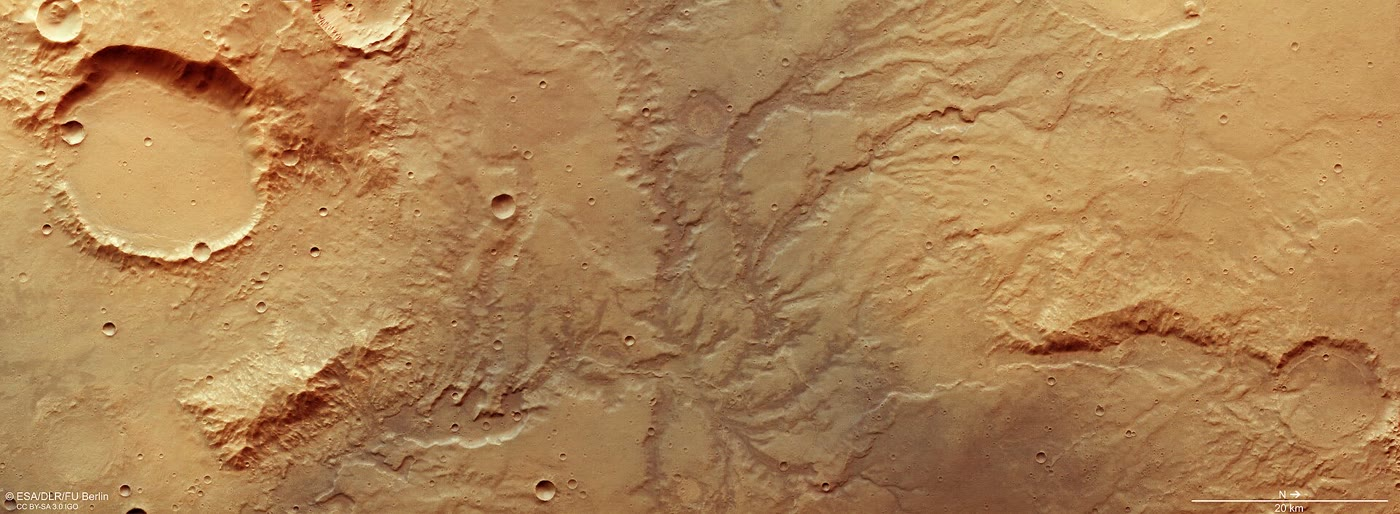
\includegraphics[width=\linewidth]{images/book5/b3-mars-valley-network.jpg}
\par\smallskip{\small Een netwerk van uitgedroogde dalen op Mars, gezien door de
camera van Mars Express op ongeveer \qty{14}{m} per pixel, nabij \ang{17}\,ZB,
\ang{66}\,OL; het noorden ligt naar rechts, en de schaalbalk is \qty{20}{km}.
Zijrivieren komen stroomafwaarts samen in grotere dalen, het patroon van een
afwateringsnetwerk. Beeld ESA/DLR/FU Berlin, CC BY-SA 3.0 IGO.}\label{fig:b3:planetary-atmospheres:valleys}
\end{omfigure}
% ledger: photo:b3-mars-valley-network

De dalen en de stroomgeulen van Mars vereisen, volgens geologische schattingen,
een wereldwijde waterlaag van 100 tot \qty{1500}{m} diep, tegenover 3 tot
\qty{25}{m} in zijn huidige ijs en atmosfeer. Veel van de rest is de ruimte in gegaan. Het
baanvaartuig MAVEN mat dat de zonnewind gas van Mars afstript, ongeveer
\qty{100}{g} per seconde, driekwart ervan in de staart
achter de planeet, waar de zonnewind stroomt, en een kwart in een pluim
boven de polen; tijdens de
zonnestormen van maart 2015 versnelde het verlies, en het was waarschijnlijk veel
sneller toen de jonge Zon actiever was. Mars verliest ook waterstof, ongeveer
\num{3e26} atomen per seconde gemiddeld vandaag: volgehouden gedurende vier miljard
jaar, een verlies dat slechts een wereldwijde waterlaag van ongeveer \qty{4}{m} diep oplevert.
% ledger: gilli25:h-loss, lasp:maven

Het tempo was niet altijd dat van vandaag. De schuinte van Mars, \ang{25.2}
nu, heeft over de laatste 250 miljoen jaar geschommeld tussen 0 en \ang{66},
rond een gemiddelde nabij \ang{35}, terwijl die van de Aarde nauwelijks meer dan een
graad varieert. De beweging is chaotisch en laat zich over miljarden
jaren niet terugrekenen; elliptische kraters, door schampende inslagen gevormd, waarvan de oriëntaties
de schuinte vastleggen, wijzen op een gemiddelde tussen ongeveer 10 en \ang{30} over
de laatste 3.5 miljard jaar of zo. Bij een grote schuinte warmt de zomerpool op,
meer waterdamp stijgt op, en klimaatmodellen geven een verlies van waterstof dat
twintig keer sneller verloopt: over de geschiedenis van Mars een laag van de orde van
\qty{80}{m}.
% ledger: planet:Mars.obliq, gilli25:obliquity, holo18:obliquity, gilli25:h-loss

\section{Titan: een methaancyclus}\label{sec:b3:planetary-atmospheres:titan}

Titan, een maan die kleiner is dan Mars, heeft een dikkere atmosfeer dan de Aarde:
met aan het oppervlak een druk die ongeveer 60\,\% hoger is, bij \qty{-179}{\degreeCelsius}.
De atmosfeer bestaat voor ongeveer 95\,\% uit stikstof en 5\,\% uit methaan, en omdat de
zwaartekracht van de maan zwak is, reikt de atmosfeer tien keer zo hoog als die van de Aarde, tot
bijna \qty{600}{km}. Ultraviolet licht splitst het methaan en de stikstof
hoog in de atmosfeer; de brokstukken recombineren tot een oranje waas van zwaardere
koolwaterstoffen die het oppervlak voor zichtbaar licht verbergen. Onder de waas
speelt methaan de rol van water: het condenseert tot wolken, regent, snijdt
rivierbeddingen uit en vult meren en zeeën van methaan en ethaan.
% ledger: nasa:titan-surface, nasa:titan-facts

\begin{omfigure}
\centering
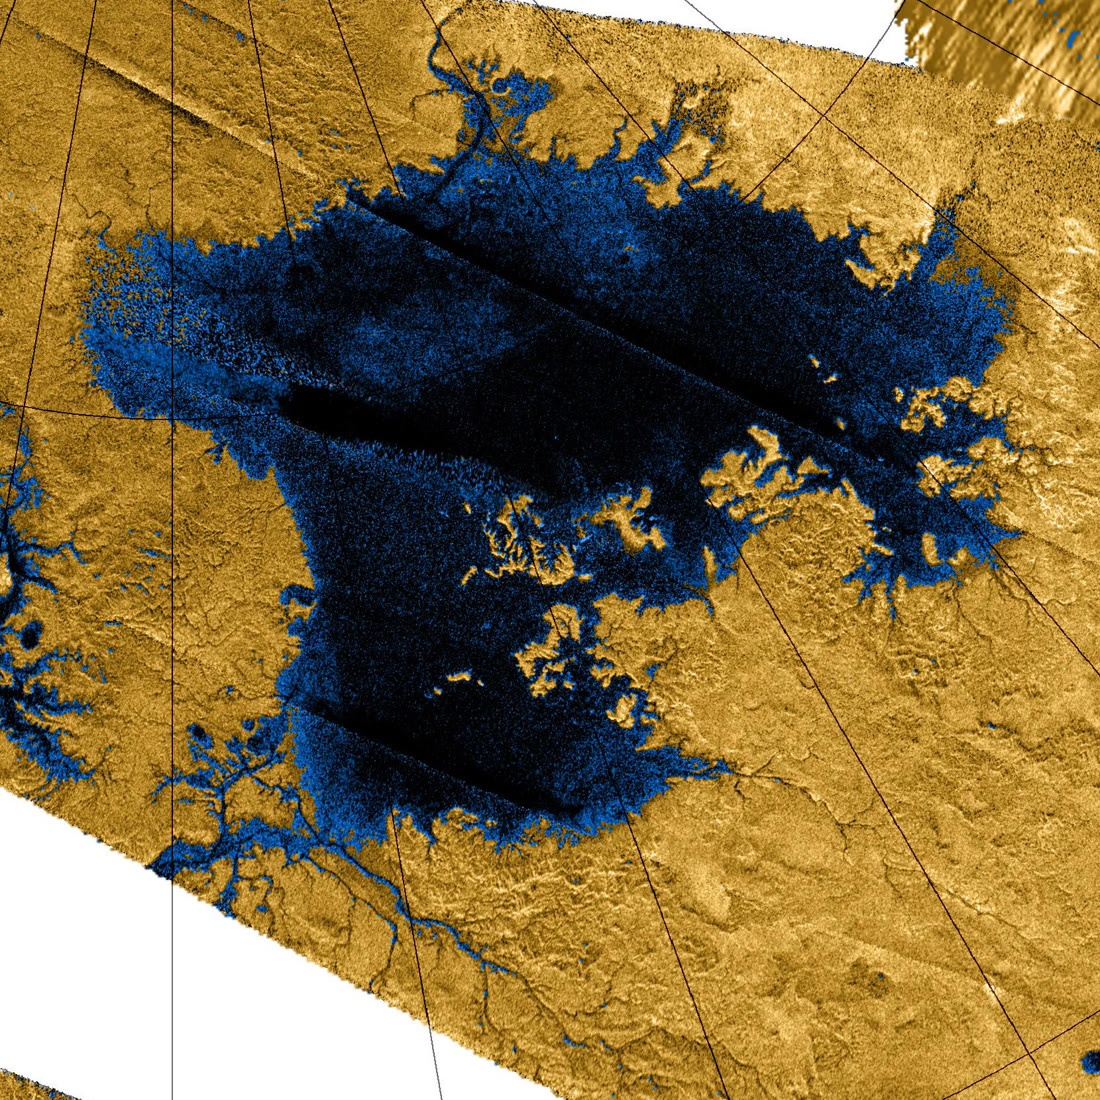
\includegraphics[width=0.5\linewidth]{images/book5/b3-ligeia-mare.jpg}
\par\smallskip{\small Ligeia Mare, een zee nabij de noordpool van Titan, in een
valskleurenmozaïek van Cassini-radarbeelden: kenmerken waarvan wordt aangenomen dat ze
vloeibaar zijn, in blauw en zwart, vaste grond bruin gekleurd, met baaien, eilanden
en vermoedelijke netwerken van zijrivieren. Van de ongeveer 400 meren en zeeën in het
gekarteerde noorden, die groter zijn dan \qty{26000}{km^2}, beslaan 70\,\% van het oppervlak.
NASA/JPL/USGS, publiek domein.}\label{fig:b3:planetary-atmospheres:ligeia}
\end{omfigure}
% ledger: photo:b3-ligeia-mare

Of een vloeistof aan een oppervlak kan liggen, hangt af van het fasediagram en van
de druk en temperatuur daar. Het oppervlak van Titan ligt net boven het
tripelpunt van methaan, \qty{90.67}{K} en \qty{0.117}{bar}, en onder
het kritieke punt: vloeibaar methaan is mogelijk, en methaan bij 5\,\% van
\qty{1.6}{bar} zit niet ver van verzadiging. Het oppervlak van Mars ligt nabij
het tripelpunt van water, dat van de Aarde ruim binnen het vloeistofgebied, en
dat van Venus boven de kritieke temperatuur van water, \qty{647}{K}, waar geen
vloeistof helemaal kan bestaan.
% ledger: nist:methane-phase, iapws:triple-critical, nasa:titan-surface

\begin{omfigure}
\centering
\begin{tikzpicture}
\begin{axis}[width=0.8\linewidth, height=0.52\linewidth,
  xmin=60, xmax=800, ymin=1e-4, ymax=1000, ymode=log,
  xlabel={temperatuur (\unit{K})}, ylabel={druk (\unit{bar})},
  tick label style={font=\scriptsize}, label style={font=\small}]
\addplot[thick, omDef] table[x=T, y=p_bar] {figdata/out/bachelor-3-habitability-water.dat};
\addplot[thick, omDef, dashed] table[x=T, y=p_bar] {figdata/out/bachelor-3-habitability-ice.dat};
\addplot[thick, orange!80!black] table[x=T, y=p_bar] {figdata/out/bachelor-3-habitability-methane.dat};
\addplot[only marks, mark=*, mark size=1.6pt, omDef] coordinates {(273.16,0.00611657) (647.096,220.64)};
\addplot[only marks, mark=*, mark size=1.6pt, orange!80!black] coordinates {(90.67,0.1169) (190.6,46.1)};
\addplot[only marks, mark=square*, mark size=2.2pt, black] table[x=T, y=p_bar] {figdata/out/bachelor-3-habitability-bodies.dat};
\node[font=\scriptsize, anchor=south] at (axis cs:737,110) {Venus};
\node[font=\scriptsize, anchor=west] at (axis cs:300,1.0) {Aarde};
\node[font=\scriptsize, anchor=north] at (axis cs:214,0.0045) {Mars};
\node[font=\scriptsize, anchor=south] at (axis cs:94,2.2) {Titan};
\node[font=\scriptsize, omDef, anchor=west] at (axis cs:420,3) {water: vloeibaar boven, damp onder};
\node[font=\scriptsize, omDef, anchor=north west] at (axis cs:205,0.0012) {ijs};
\node[font=\scriptsize, orange!80!black, anchor=west] at (axis cs:196,46) {methaan};
\node[font=\scriptsize, omDef, anchor=south east] at (axis cs:640,230) {kritiek punt};
\end{axis}
\end{tikzpicture}
\par\smallskip{\small De grenzen tussen damp en gecondenseerd water
(blauw: vloeistof--damp, van het tripelpunt tot het kritieke punt;
gestippeld: ijs--damp) en tussen vloeibaar methaan en zijn damp (oranje),
met de gemiddelde oppervlaktetoestanden van Venus, de Aarde, Mars en Titan
(vierkantjes). Een vloeistof kan liggen op een oppervlak waarvan de druk boven de
kromme van die vloeistof ligt, tussen zijn tripel- en kritieke
temperatuur.}\label{fig:b3:planetary-atmospheres:phases}
\end{omfigure}
% ledger: iapws:vapour-pressure, iapws4:sublimation, iapws:triple-critical, nist:methane-phase, nasa:venus-atm, planet:Earth.Tmean, planet:Earth.psurf, nasa:mars-atm, nasa:titan-surface

Titan houdt zijn stikstof gemakkelijk vast: bij zijn \omterm{def:b3:planetary-atmospheres:exobase}{exobasis} $\lambda = 41$ voor
stikstof. Zijn waterstof, bij $\lambda$ rond 1.5, ontsnapt bijna vrij, en
de ontsnapping van moleculaire waterstof wordt lager bepaald door de begrenzende flux
door de \omterm{def:b3:planetary-atmospheres:hydrodynamic}{homopauze}, zoals op de Aarde. De zware verbindingen die uit het
gebroken methaan ontstaan, bezinken naar het oppervlak, waar ze het zand vormen van uitgestrekte
velden van duinen.
% ledger: gronoff:jeans-table, gronoff:diffusion, nasa:titan-surface

\section{Planetaire bewoonbaarheid}\label{sec:b3:planetary-atmospheres:habitability}

De bewoonbare zone uit de schoolboeken is het bereik van afstanden tot een
ster waarop een planeet zoals de Aarde vloeibaar water aan zijn
oppervlak kan houden. De randen ervan zijn de grenzen die in dit hoofdstuk aan bod komen.

\begin{definition}[Planetaire bewoonbaarheid]\label{def:b3:planetary-atmospheres:habitability}
De \emph{planetaire bewoonbaarheid}\index{planetaire bewoonbaarheid} van een
planeet is haar vermogen om vloeibaar water aan het oppervlak over
geologische tijd te houden: ze ontvangt een stellaire flux binnen de grenzen van de
bewoonbare zone; ze houdt haar atmosfeer en haar water vast tegen
ontsnapping, en een langdurige koolstofcyclus regelt haar klimaat.
\end{definition}

De binnenrand van de bewoonbare zone is het vochtige of het \omterm{def:b3:planetary-atmospheres:runaway}{op hol geslagen
broeikaseffect}: een aardachtige planeet rond de Zon wordt vochtig bij
\qty{0.99}{au} en slaat op hol bij \qty{0.97}{au}. De buitenrand is het
\emph{maximaal broeikaseffect}: koolstofdioxide toevoegen verwarmt een planeet alleen tot
het extra gas meer zonlicht terugverstrooit dan zijn broeikaseffect
oplevert; rond de Zon gebeurt dat bij
\qty{1.70}{au}, bij ongeveer \qty{8}{bar} koolstofdioxide. Dat zijn
conservatieve randen, berekend zonder wolken. Twee empirische randen zijn breder:
Venus lijkt minstens een miljard jaar geen oppervlaktewater te hebben gehad,
toen het 1.76 keer het huidige zonlicht van de Aarde ontving (\qty{0.75}{au});
Mars had stromend water toen het 0.32 keer dat zonlicht ontving, als de
valleien 3.8 miljard jaar oud zijn (\qty{1.77}{au}). Rond koelere sterren komen dezelfde grenzen
bij lagere fluxen, omdat hun roodere licht minder wordt verstrooid en meer wordt
geabsorbeerd door water en koolstofdioxide.
% ledger: kopparapu13:runaway, kopparapu13:outer, kopparapu13:hz-fit

\begin{omfigure}
\centering
\begin{tikzpicture}
\begin{axis}[width=0.8\linewidth, height=0.5\linewidth,
  xmin=0, xmax=2.1, ymin=2600, ymax=7200, x dir=reverse,
  xlabel={stellaire flux ontvangen / die van de Aarde nu},
  ylabel={stellaire temperatuur (\unit{K})},
  tick label style={font=\scriptsize}, label style={font=\small},
  legend style={font=\scriptsize, at={(0.5,-0.24)}, anchor=north, legend columns=2, draw=none}]
\addplot[name path=mg, thick, omDef] table[x=mg, y=Teff] {figdata/out/bachelor-3-habitability-hz.dat};
\addlegendentry{vochtig broeikaseffect}
\addplot[name path=maxg, thick, red!70!black] table[x=maxg, y=Teff] {figdata/out/bachelor-3-habitability-hz.dat};
\addlegendentry{maximaal broeikaseffect}
\addplot[thin, omDef, dashed] table[x=rg, y=Teff] {figdata/out/bachelor-3-habitability-hz.dat};
\addlegendentry{op hol geslagen broeikaseffect}
\addplot[thin, black!60, densely dotted] table[x=rv, y=Teff] {figdata/out/bachelor-3-habitability-hz.dat};
\addlegendentry{recent Venus, vroeg Mars}
\addplot[thin, black!60, densely dotted, forget plot] table[x=em, y=Teff] {figdata/out/bachelor-3-habitability-hz.dat};
\addplot[green!30, opacity=0.5, forget plot] fill between[of=mg and maxg];
\addplot[only marks, mark=*, mark size=2pt, black, forget plot] coordinates {(1.911,5780) (1.0,5780) (0.431,5780)};
\node[font=\scriptsize, anchor=south] at (axis cs:1.911,5800) {Venus};
\node[font=\scriptsize, anchor=west, xshift=2pt] at (axis cs:1.0,5780) {Aarde};
\node[font=\scriptsize, anchor=east, xshift=-2pt] at (axis cs:0.431,5780) {Mars};
\end{axis}
\end{tikzpicture}
\par\smallskip{\small De bewoonbare zone van een aardachtige planeet, uitgedrukt als de
stellaire flux die hij ontvangt, uitgezet tegen de temperatuur van zijn ster (gearceerd:
tussen het vochtige broeikaseffect en het maximale broeikaseffect). Stippellijnen: de
empirische grenzen afgeleid uit recent Venus en vroeg Mars. De fits zijn
die van een wolkenvrij klimaatmodel, geldig van 2600 tot
\qty{7200}{K}.}\label{fig:b3:planetary-atmospheres:hz}
\end{omfigure}
% ledger: kopparapu13:hz-fit, nasa:venus, nasa:mars

Afstand alleen is niet genoeg. Een planeet moet zijn atmosfeer vasthouden: een kleine
of hete, waarvan de \omterm{def:b3:planetary-atmospheres:jeans-escape}{ontsnappingsparameter} laag is, verliest zijn waterstof en daarmee
zijn water, en een planeet in een \omterm{def:b3:planetary-atmospheres:runaway}{vochtig broeikaseffect} droogt van bovenaf uit. Hij
moet ook zijn klimaat over miljarden jaren stabiel houden, terwijl zijn ster
helderder wordt: op de Aarde vormt de silicaatverwering-thermostaat van de
langetermijnkoolstofcyclus trekt koolstofdioxide omlaag wanneer het klimaat opwarmt
en laat het zich opbouwen wanneer het afkoelt. Op Venus, zonder platentektoniek,
uitgegast koolstofdioxide heeft nooit een weg terug in de gesteenten gevonden en
is in de lucht opgehoopt; het bevat nu ongeveer evenveel koolstofdioxide als de
Aarde in carbonaatgesteenten heeft vastgelegd. Of een magnetisch veld een
atmosfeer beschermt, is omstreden: het schermt de bovenste atmosfeer af van de
zonnewind, maar het opent ook andere ontsnappingswegen, zoals de uitstroom van ionen
nabij de polen, en de bewoonbaarheid van een planeet valt niet af te lezen
uit zijn plaats in de bewoonbare zone alleen.
% ledger: arney18:venus-loss, gronoff21:magnetic, gronoff:nonthermal

\section{Oefeningen}

\begin{exercise}[$\star$]\label{exo:b3:planetary-atmospheres:1}
Bereken de schaalhoogte $H = RT/Mg$ vlak boven het oppervlak van Venus
(\qty{737}{K}, koolstofdioxide met molaire massa \qty{44.01}{g.mol^{-1}},
$g = \qty{8.87}{m.s^{-2}}$), van de Aarde (\qty{288}{K},
\qty{28.97}{g.mol^{-1}}, \qty{9.80}{m.s^{-2}}), van Mars (\qty{214}{K},
\qty{43.34}{g.mol^{-1}}, \qty{3.71}{m.s^{-2}}) en van Titan (\qty{94}{K},
\qty{28.0}{g.mol^{-1}}, \qty{1.35}{m.s^{-2}}). Welke atmosfeer is de
meest uitgebreide, en waarom?
\end{exercise}

\begin{exercise}[$\star$]\label{exo:b3:planetary-atmospheres:2}
De \omterm{def:b3:planetary-atmospheres:exobase}{exobasis} van de Aarde ligt op \qty{500}{km} (straal \qty{6878}{km});
de temperatuur ervan varieert van 800 tot \qty{1600}{K} over de zonnecyclus.
Neem de massa van de Aarde als \qty{5.97e24}{kg}. Bereken de \omterm{def:b3:planetary-atmospheres:jeans-escape}{ontsnappingsparameter}
van waterstofatomen bij beide temperaturen, en de ontsnappende fractie
$(1 + \lambda)e^{-\lambda}$. Met welke factor verandert de zonnecyclus die?
\end{exercise}

\begin{exercise}[$\star$]\label{exo:b3:planetary-atmospheres:3}
Rond de Zon wordt een aardachtige planeet vochtig bij de flux $S_\mathrm{eff}
= 1.014$, raakt op hol bij 1.0512 en bereikt het maximale broeikaseffect bij 0.3438
(fluxen ten opzichte van die van de Aarde). (a)~Bereken de drie afstanden, in
astronomische eenheden. (b)~Venus en Mars ontvangen respectievelijk 1.91 en 0.43 keer
het zonlicht van de Aarde. Plaats ze.
\end{exercise}

\begin{exercise}[$\star$]\label{exo:b3:planetary-atmospheres:4}
De dampdruk van vloeibaar methaan is $\log_{10}(p/\unit{bar}) = 3.9895 -
443.028/(T/\unit{K} - 0.49)$. (a)~Bereken die aan het oppervlak van Titan,
\qty{94.15}{K}. (b)~Methaan vormt 5\,\% van de lucht van Titan bij \qty{1.6}{bar}.
Bereken de partiële druk ervan en de relatieve luchtvochtigheid. (c)~Wat suggereert
het resultaat over verdamping uit de zeeën van Titan?
\end{exercise}

\begin{exercise}[$\star\star$]\label{exo:b3:planetary-atmospheres:5}
Aan de \omterm{def:b3:planetary-atmospheres:exobase}{exobasis} van de Aarde (\qty{1000}{K}, $\lambda = 7.02$ voor waterstof),
bereken de \omterm{def:b3:planetary-atmospheres:jeans-escape}{ontsnappingsparameter} van deuterium, de thermische snelheid ervan ten opzichte van
die van waterstof en de verhouding van de Jeans-flux per atoom, D ten opzichte van H. Is
\omterm{def:b3:planetary-atmospheres:jeans-escape}{Jeans-ontsnapping} een sterk isotopenfilter?
\end{exercise}

\begin{exercise}[$\star\star$]\label{exo:b3:planetary-atmospheres:6}
De verhouding D/H van het water van Venus is \num{0.016}; die van oceaanwater op
de Aarde is \num{1.5575e-4}. (a)~Bereken de verrijking. (b)~Zonder enige
ontsnapping van deuterium, wat is de kleinste vroegere voorraad water
van Venus, gegeven \qty{6e15}{kg} vandaag? Welke diepte zou die opleveren, uitgespreid over
het oppervlak van de planeet van \qty{4.60e14}{m^2}? (c)~Welke krimp van het reservoir zou
\omterm{def:b3:planetary-atmospheres:hydrodynamic}{diffusiebeperkte ontsnapping}, met $\alpha = 0.8$, vereisen? Trek een conclusie.
\end{exercise}

\begin{exercise}[$\star\star$]\label{exo:b3:planetary-atmospheres:7}
Mars, met een straal van \qty{3389.5}{km}, verliest ongeveer \num{3e26} waterstofatomen
per seconde. (a)~Als elk paar atomen afkomstig was van een watermolecuul, welke
wereldwijde waterlaag verwijdert het verlies dan in vier miljard jaar?
(b)~Dezelfde vraag bij \num{6e27} atomen per seconde, het tempo van een hoge
obliquiteit. (c)~Vergelijk met de 100 tot \qty{1500}{m} die de valleien en
geulen nodig hebben.
\end{exercise}

\begin{exercise}[$\star\star$]\label{exo:b3:planetary-atmospheres:8}
(a)~Bereken de massa van de atmosfeer van Mars uit de gemiddelde
oppervlaktedruk, \qty{636}{Pa}, de zwaartekracht, \qty{3.71}{m.s^{-2}}, en
de straal. (b)~De zonnewind verwijdert ongeveer \qty{100}{g} gas per seconde. Welke massa verwijdert dat in vier miljard jaar, en in hoeveel tijd zou
het de huidige atmosfeer verwijderen? (c)~Waarom is dat een onderschatting van het
verlies in het verleden?
past loss?
\end{exercise}

\begin{exercise}[$\star\star$]\label{exo:b3:planetary-atmospheres:9}
Een aardachtige planeet met een wolkenvrije stoomatmosfeer weerkaatst 19.3\,\% van
het zonlicht dat hij ontvangt; zijn infrarode uitstraling kan
\qty{291}{W.m^{-2}} niet overschrijden. (a)~Boven welke zonnestraling, in watt per vierkante
meter en ten opzichte van de \qty{1361}{W.m^{-2}} van de Aarde, loopt hij op hol?
(b)~Vergelijk met Venus vandaag, \qty{2601}{W.m^{-2}}, en met een jonge Venus
onder een Zon op 70\,\% van zijn huidige lichtkracht. (c)~Waarom is de
conclusie voor de jonge Venus niet definitief?
\end{exercise}

\begin{exercise}[$\star\star\star$]\label{exo:b3:planetary-atmospheres:10}
Een modelthermosfeer van atomair zuurstof is isotherm bij \qty{1000}{K}, met
$n = \qty{1e16}{m^{-3}}$ op \qty{200}{km}; neem $g =
\qty{9.21}{m.s^{-2}}$ op die hoogte en een botsingsdoorsnede
$\sigma_c = \qty{3e-19}{m^2}$. (a)~Bereken de schaalhoogte van het zuurstof.
(b)~Bereken de dichtheid aan de \omterm{def:b3:planetary-atmospheres:exobase}{exobasis} en de hoogte van de \omterm{def:b3:planetary-atmospheres:exobase}{exobasis}.
(c)~De zwaartekracht neemt af met de hoogte. Verplaatst dat de \omterm{def:b3:planetary-atmospheres:exobase}{exobasis} omhoog of
omlaag?
\end{exercise}

\begin{exercise}[$\star\star\star$]\label{exo:b3:planetary-atmospheres:11}
(a)~Stel dat de stratosfeer van de Aarde vochtig werd, met een mengverhouding van
waterdamp van \num{3e-3} (geteld als $\ce{H2}$). Neem de diffusiegrens
$\num{3.0e13}\,f$ moleculen $\ce{H2}$ per vierkante centimeter en
per seconde, bij \qty{200}{K}, bereken het waterstofverlies van de hele
Aarde (straal \qty{6371}{km}). (b)~Hoe lang zou een oceaan,
\qty{1.4e24}{g} water, het uithouden? Vergelijk met de ouderdom van de Aarde.
\end{exercise}

\begin{exercise}[$\star\star\star$]\label{exo:b3:planetary-atmospheres:12}
In een bovenatmosfeer van zuivere stoom die als grijs gas absorbeert met $\kappa =
\qty{0.005}{m^2.kg^{-1}}$, op een planeet met $g = \qty{9.81}{m.s^{-2}}$
en $D = 1.66$: (a)~bereken de druk $p_1$ van het stralende niveau;
(b)~met $p_\mathrm{sat}(T) = \qty{611.657}{Pa}\,\exp[(L/R_v)(1/T_t -
1/T)]$, $L = \qty{2.5e6}{J.kg^{-1}}$, $R_v = \qty{461.5}{J.kg^{-1}.K^{-1}}$,
$T_t = \qty{273.16}{K}$, bereken de temperatuur ervan en de stralingsgrens.
(c)~De lijn-voor-lijngrens is \qty{291}{W.m^{-2}}. Moet het effectieve
$\kappa$ van echte waterdamp groter of kleiner zijn?
\end{exercise}

\section{Probleem: Zal Kepos zijn water behouden?}

\begin{problem}[{Weekendprobleem --- ontsnapping en bewoonbaarheid van een verzonnen
oceaanplaneet}]
\label{pb:b3:planetary-atmospheres:1}
Kepos is een verzonnen planeet met een massa van \qty{5.2e24}{kg} en een
straal van \qty{6200}{km}, met oceanen en een atmosfeer van stikstof en
koolstofdioxide. Hij draait op \qty{0.60}{au} om een ster met een lichtkracht van 0.30 maal die van de
Zon en een effectieve temperatuur van \qty{4800}{K}. Zijn \omterm{def:b3:planetary-atmospheres:exobase}{exobasis} ligt
\qty{500}{km} boven het oppervlak, bij \qty{1400}{K}, met
\qty{2e11}{m^{-3}} waterstofatomen; zijn \omterm{def:b3:planetary-atmospheres:hydrodynamic}{homopauze} ligt bij \qty{200}{K},
waar koolstofdioxide domineert en waar waterstof in al zijn vormen een
mengverhouding $f = \num{1e-3}$ heeft, geteld als $\ce{H2}$. Een Aardse oceaan is
\qty{1.4e24}{g} water.

\medskip\noindent\textbf{Deel I --- De exobasis.}
\begin{enumerate}
\item Bereken de zwaartekracht aan het oppervlak en de gemiddelde dichtheid van Kepos.
\item Bereken de ontsnappingssnelheid aan de \omterm{def:b3:planetary-atmospheres:exobase}{exobasis}.
\item Bereken de thermische snelheid $u = \sqrt{2kT/m}$ van waterstof-, helium- en
  zuurstofatomen aan de \omterm{def:b3:planetary-atmospheres:exobase}{exobasis}.
\item Bereken hun \omterm{def:b3:planetary-atmospheres:jeans-escape}{ontsnappingsparameters}.
\item Welke van hen kunnen door \omterm{def:b3:planetary-atmospheres:jeans-escape}{Jeans-ontsnapping} met een significant tempo ontsnappen?
  Komt er een dicht bij het hydrodynamische regime?
\item Tijdens een actieve jeugd van zijn ster kan de \omterm{def:b3:planetary-atmospheres:exobase}{exobasis} van Kepos
  \qty{3000}{K} hebben bereikt. Wat was toen de \omterm{def:b3:planetary-atmospheres:jeans-escape}{ontsnappingsparameter} van waterstof,
  en wat suggereert dat?
\end{enumerate}

\medskip\noindent\textbf{Deel II --- Jeans-ontsnapping van waterstof.}
\begin{enumerate}[resume]
\item Bereken de ontsnappende fractie $(1 + \lambda)e^{-\lambda}$ voor
  waterstof.
\item Bereken de Jeans-flux van waterstof, per vierkante meter en per seconde.
\item Bereken het aantal waterstofatomen dat de hele \omterm{def:b3:planetary-atmospheres:exobase}{exobasis} verlaat
  per seconde.
\item Hoeveel waterstofatomen bevat een Aardse oceaan?
\item Hoelang zou Kepos er met dit tempo over doen om ze te verliezen?
\item Bereken de \omterm{def:b3:planetary-atmospheres:jeans-escape}{ontsnappingsparameter} van deuterium en de ontsnappingsefficiëntie
  ten opzichte van waterstof, per atoom.
\end{enumerate}

\medskip\noindent\textbf{Deel III --- De diffusiegrens.}
\begin{enumerate}[resume]
\item Bereken de schaalhoogte van koolstofdioxide aan de \omterm{def:b3:planetary-atmospheres:hydrodynamic}{homopauze}.
\item De binaire diffusieparameter van waterstof in koolstofdioxide is
  $b = \qty{1.2e19}{cm^{-1}.s^{-1}}$ bij \qty{200}{K}. Bereken de
  diffusiebeperkte flux van $\ce{H2}$, per vierkante meter en per seconde.
\item Controleer dit tegen de grens van de Aarde, $\num{3.0e13}\,f$ moleculen per
  vierkante centimeter en per seconde, geschaald met de zwaartekracht.
\item Bereken het aantal waterstofatomen dat de diffusiegrens per seconde kan
  leveren aan de bovenatmosfeer van de hele planeet (neem het
  oppervlak van de planeet).
\item Vergelijk met vraag~9. Welk proces beperkt de ontsnapping, en wat
  gebeurt er met het waterstof van de thermosfeer?
\item Welke dichtheid van waterstof aan de \omterm{def:b3:planetary-atmospheres:exobase}{exobasis} zou ervoor zorgen dat
  \omterm{def:b3:planetary-atmospheres:jeans-escape}{Jeans-ontsnapping} de hele aanvoer kan afvoeren?
\item Hoelang zou Kepos erover doen om een Aardse oceaan waterstof te verliezen
  bij de diffusiegrens?
\end{enumerate}

\medskip\noindent\textbf{Deel IV --- Ligt Kepos in de bewoonbare zone?}
\begin{enumerate}[resume]
\item Bereken de stellaire flux die Kepos ontvangt, ten opzichte van die van de Aarde.
\item Voor een ster van \qty{4800}{K} ligt de limiet van het vochtige broeikaseffect bij
  $S_\mathrm{eff} = 0.939$ en het maximale broeikaseffect bij 0.290. Bereken de
  randen van de bewoonbare zone, in astronomische eenheden, en plaats Kepos.
\item Met welke factor moet de ster helderder worden voordat Kepos de binnenrand
  bereikt?
\item Bereken, met een albedo van 0.3, het zonlicht dat Kepos per vierkante
  meter absorbeert, en zijn evenwichtstemperatuur. Vergelijk met de \omterm{def:b3:planetary-atmospheres:runaway}{limiet van het
  op hol geslagen broeikaseffect}.
\item Als een warmer klimaat de stratosfeer van Kepos vochtig maakte, met
  $f = \num{3e-3}$, hoelang zou een Aardse oceaan het dan uithouden?
\item Geef de tijd die Kepos nodig heeft om een Aardse oceaan waterstof te verliezen door
  \omterm{def:b3:planetary-atmospheres:hydrodynamic}{diffusiebeperkte ontsnapping} met $f = \num{1e-3}$, in miljarden jaren, op
  twee significante cijfers.
\end{enumerate}
\end{problem}
% ledger: zahnle19:diffusion, kopparapu13:hz-fit, kopparapu13:runaway, gronoff:jeans, const:G, const:kB, const:NA
